
\begin{frame}{TDKENO Solution Method}

\begin{itemize}[<+-| alert@+>]
    \item Hybrid method of solving transport equation 
    \item $T(t)$ solved deterministically -- point kinetics
    \item $ \Phi(r,E,\Omega,t)$ solved stochastically -- flux shape
    \item Coupled equations solved on different time intervals
\end{itemize}
\begin{figure}
    \centering
    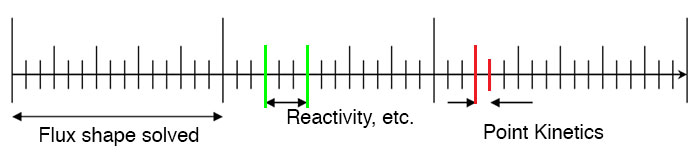
\includegraphics[width=10cm]{figures/time_scale_COLOR.jpg}
    \label{fig:time_scale}
\end{figure}

%\begin{itemize}[<+-| alert@+>]
%    \item that is actually not enough, we need to include sub-resolution physics %(cooling, star formation, feedback processes, ...) and we would like to have %radiative transport as well
%        \tikz[remember picture] \node[coordinate] (n1) {};
%\end{itemize}

%\begin{tikzpicture}[remember picture,overlay]   %% use here too
%        \path[draw=magenta,thick,->]<3-> ([yshift=2mm]n1.north) to [out=0, %in=0,distance=1in] (t1.east);
%\end{tikzpicture}

\end{frame}